% LaTeX template for Lab Reports
% Copyright (C) 2014 Julian Coy

%% CHANGE REPORT TITLE HERE
\newcommand{\reporttitle}{
 AMD Crossfire
}

%% HEADER/PREAMBLE INFORMATION

% "The font should be 11pt Times New Roman"
\documentclass[11pt]{report}
\usepackage[T1]{fontenc}
\usepackage[utf8]{inputenc}

\usepackage{mathptmx}               

% "The body of the paper should use 1" margins on all sides."
\usepackage[margin=1in]{geometry}

% "Pages must be numbered, starting with 1 on the first page in the body of the report.
% The cover page should not be numbered. 
% Page numbers should be in the bottom-right corner of the page."
\usepackage{fancyhdr}
\pagestyle{fancy}
\fancyhead{}
\fancyfoot{}
\renewcommand{\headrulewidth}{0pt}
\fancyfoot[R]{\thepage}

% Set up customized spacing
\usepackage{setspace}

% Allows for Trademark Symbols
\usepackage{textcomp}

% Remove spacing between items in lists
\usepackage{enumitem}

% Remove extra spacing between titles of sections and subsections
\usepackage{titlesec}
\titlespacing\section{0pt}{10pt}{10pt}
\titlespacing\subsection{0pt}{10pt}{10pt}
\titlespacing\subsubsection{0pt}{0pt plus 4pt minus 2pt}{0pt plus 2pt minus 2pt}

% Setup the specialized chapter section for the Abstract
\titlespacing\chapter{0pt}{0pt plus 4pt minus 2pt}{0pt plus 2pt minus 2pt}
\titleformat{\chapter}[block]{\centering\Huge}{}{}{}{}

% Set up BibTeX integration using IEEE citation format
\usepackage{cite}
\bibliographystyle{ieeetr}
\usepackage{url}

% Set bibliography to have a section header rather than chapter header
\makeatletter
\renewenvironment{thebibliography}[1]
     {\chapter*{\scshape Bibliography}% <-- this line was changed from \chapter* to \section*
      \vspace{45px}
      \@mkboth{\MakeUppercase\bibname}{\MakeUppercase\bibname}%
      \list{\@biblabel{\@arabic\c@enumiv}}%
           {\settowidth\labelwidth{\@biblabel{#1}}%
            \leftmargin\labelwidth
            \advance\leftmargin\labelsep
            \@openbib@code
            \usecounter{enumiv}%
            \let\p@enumiv\@empty
            \renewcommand\theenumiv{\@arabic\c@enumiv}}%
      \sloppy
      \clubpenalty4000
      \@clubpenalty \clubpenalty
      \widowpenalty4000%
      \sfcode`\.\@m}
     {\def\@noitemerr
       {\@latex@warning{Empty `thebibliography' environment}}%
      \endlist}
\makeatother

% Set up math
\usepackage{amsmath}
\usepackage{amsfonts}
\usepackage{amssymb}

% Set up graphics
\usepackage{graphicx}
\usepackage{float}

% Set up tables
\usepackage{tabularx}
\usepackage{booktabs}

% Set up code blocks
% or not...

\usepackage{listings}
\usepackage{color}

\definecolor{dkgreen}{rgb}{0,0.6,0}
\definecolor{gray}{rgb}{0.5,0.5,0.5}
\definecolor{mauve}{rgb}{0.58,0,0.82}

\lstset{frame=tb,
  language=VHDL,
  aboveskip=3mm,
  belowskip=3mm,
  showstringspaces=false,
  columns=flexible,
  basicstyle={\small\ttfamily},
  numbers=none,
  numberstyle=\tiny\color{gray},
  keywordstyle=\color{blue},
  commentstyle=\color{dkgreen},
  stringstyle=\color{mauve},
  breaklines=true,
  breakatwhitespace=true
  tabsize=3
}

%% START OF DOCUMENT

\begin{document}

% "The main body of text should use 1.5 spacing"
\begin{spacing}{1.5}

% Suppress page numbering on first page
\thispagestyle{empty}

\begin{scshape}

% Title
% "The title should be centered and written in approximately 22pt font."
\vspace*{30pt}
{
\Huge
\begin{center}
    \reporttitle
\end{center}
}
\vspace{30pt}

% Team Number
% "The Team number should be centered and written several lines below the title and should use a
% similar size font as the title."
{
\Large
\begin{center}
  Prepared for Dr. Adam Hoover's ECE468 \\
  Embedded Computing
\end{center}
}
\vspace{30pt}
% Team Members
% "Directly below the team identifier, team members should be listed alphabetically by last name, one
% per line, in approximately 14pt font. The column of names should be approximately centered on
% the page, but the names within the column should be left justified (so they all start at the same
% horizontal position)."
{
\Large 
\begin{center}
  Submitted by \\
  Julian Coy \& James Jernigan
\end{center}
}
\vspace{120pt}

{
\Large
\begin{center}
  Undergraduate of Electrical \& Computer Engineering \\
  Clemson University
\end{center}
}
\vspace{30pt}

{
\Large
\begin{center}
  March 13, 2013
\end{center}
}

\end{scshape}

% New page and reset page numbering
\clearpage
\setcounter{page}{1}

%% START EDITS BELOW %%

\nocite{AMD}
\nocite{WIKI}
\nocite{THW}

\section*{\scshape Introduction}

Crossfire is a technology developed by AMD that allows for distributed graphics computing 
across multiple GPUs. First introduced in 2005, this technology is incorporated into a wide range of GPU 
products licensed and sold by AMD, both recreational and professional. The individual computing power 
of the GPUs are combined (minus overhead) allowing for speeds faster than that of even top-of-the-line 
graphics cards. This technology does have its limitations, but provides an affordable solution 
to upgrading a computer as well as a way to maximize performance with the fastest technology.
Crossfire works by using Alternate Frame Rendering (AFR) between the connected GPUs. Each 
graphics card will render an output frame in a round-robin fashion, with support up to four cards. Since 
frames are still rendered by GPUs individually, the video ram of each card is not additive in Crossfire. A 
program that needs 2GB of VRAM to run properly will not work with two 1GB cards. Frames rendered by 
GPUs not connected to the output display are transmitted to via PCI-Express or a proprietary hardware 
bridge and stored in a buffer until their turn to output. Hybrid Crossfire (or Dual Crossfire) works in a 
similar fashion, but data is processed by the integrated GPU of an AMD processor and transmitted to the 
discrete graphics card.

\section*{\scshape Analysis}

Typical performance gains in a homogenous Crossfire setup are 70-80\% boost from the second 
GPU and less from each successive card. This can create very powerful rendering capability and surpass 
the output of even the most powerful singular GPUs. In some hybrid Crossfire schemes, improvements 
of over 100\% have been seen in midrange cards with the addition of the integrated GPU. This creates 
systems that maximize performance per cost instead of just raw power.
In either case, Crossfire is meant for systems that place greater demand on graphics processing. 
This primarily falls into either video gaming or professional graphics environment (CAD, Adobe products, 
etc). It is also very beneficial when using large display resolutions such as 4k or an Eyefinity 
configuration. 
\vspace{20px}

With the array of benefits associated with the technology, Crossfire does have drawbacks. 
Crossfire is not meant for regular computer usage and will not improve the performance of CPU based 
tasks. Even for graphical programs, the performance of the technology is dependent upon the 
applications using it. Some programs may not see any gains at all. Also, graphical performance can 
actually be lessened when using low display resolutions compared to a single GPU. Another particular 
problem in the technology is a phenomenon known as micro-stuttering. It occurs when the time 
between frames output to the monitor vary significantly even with a constant average frame rate. This is 
usually due to improper load balancing between the GPUs and results in an unsmooth image. 
This micro-stuttering is one area where AMD falls short of its direct competitor, Nvidia. The 
latter has a technology called Scalable Link Interface (SLI) that is analogous to Crossfire. Although SLI 
does not see the same 70-80\% average boost with the addition of the second card, it has far less micro-
stutter. This can be seen in Figure \ref{fig:thw}. Crossfire, however, is more flexible than SLI when combining GPUs.

\vspace{30px}
\begin{figure}[H]
    \centering
    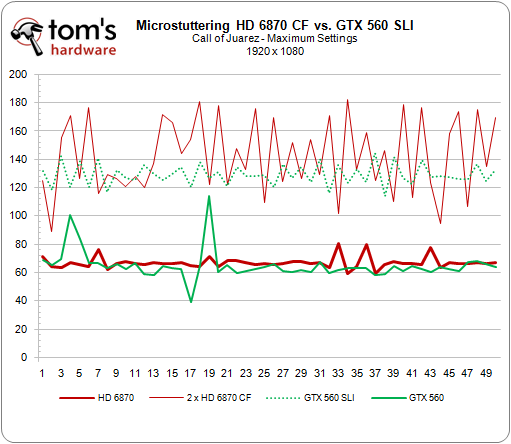
\includegraphics[width=0.6\textwidth]{fig1.png}
    \caption{Comparison of AMD HD 6870 Crossfire and Nvidia GTX 560 SLI}
    \label{fig:thw}
\end{figure}

\section*{\scshape Conclusion}

Crossfire is not appropriate for every application.  It has issues rendering low-resolution, problems with micro-stuttering,
and it is non-beneficial for CPU intensive applications.  Despite all this, Crossfire will continue to be a viable
solution for upgrading under-performing systems or for building a new top-of-the-line machine.

% Although it is not meant for every application, Crossfire will continue to be a viable solution for 
% upgrading an underperforming system or creating a new computer with the most powerful 
% specifications available.


% http://products.amd.com/en-us/graphiccardresult.aspx GPU specifications directly from AMD.

% http://en.wikipedia.org/wiki/AMD_CrossFireX History and basic information

% http://www.tomshardware.com/reviews/radeon-geforce-stutter-crossfire,2995-5.html Specific data on 
% Crossfire and SLI performance.

% Figure 1: Comparison of AMD HD 6870 Crossfire and Nvidia GTX 560 SLI

% Bibliography

\clearpage

\bibliography{citationsfile}{}

%% END EDITS HERE %%

\end{spacing}

\end{document}

%%%%%%%%%%%% Extra stuff for use later
